\documentclass[conference]{IEEEtran}

\usepackage{
	hyperref,
	graphicx,
	amssymb,
	algorithm,
	algorithmicx,
	footnote,
}
\usepackage[noend]{algpseudocode}

\renewcommand\IEEEkeywordsname{Keywords}
\newcommand*\Let[2]{\State #1 $\gets$ #2}
\algrenewcommand\algorithmicrequire{\textbf{Precondition:}}
\algrenewcommand\algorithmicensure{\textbf{Postcondition:}}

\newcommand{\backtrackarrow}{\rotatebox[origin=c]{-90}{$\curvearrowleft$}}

\newcommand{\complexity}[9]{
\begin{table}[ht]
	\begin{center}
		\begin{tabular}{l|c|c}
			\textbf{Operation} & \textbf{#1} & \textbf{#2} \\
			\hline
			\textit{StartTimer} & $O(#3)$ & $O(#4)$ \\
			\textit{PerTick} & $O(#5)$ & $O(#6)$ \\
			\textit{DeleteTimer} &  $O(#7)$ & $O(#8)$ \\
		\end{tabular}
		\linebreak
		\caption{Runtime Complexity for #9}
	\end{center}
\end{table}
}

\makesavenoteenv{tabular}
\makesavenoteenv{table}

\title{Timer Lawn: Solving the Timer Wheel Overflow Problem for Large Scale and High Throughput Systems} 


\author{
	\textsc{Adam Lev-Libfeld} \\[1ex]
%	\orcid{000-0002-3268-0851}
	\normalsize Tamar Labs \\
	\normalsize Tel-Aviv, Israel \\
	\normalsize{adam@tamarlabs.com}
}
\date{\today}

\begin{document}

\maketitle

\begin{abstract}
As the usage of Real-Time applications and algorithms rises, so does the importance of enabling large-scale, unbound algorithms to solve conventional problems with low to no latency becomes critical for product viability\cite{REND, WHT}. Timer algorithms are prevalent in the core mechanisms behind operating systems\cite{BSD}, network protocol implementation, real-time and stream processing, and several database capabilities. This paper presents a field-tested algorithm for low latency, unbound timer data structure, that improves upon the well excepted Timing Wheel algorithm. Using a set of queues mapped to by TTL instead of expiration time, the algorithm allows for a simpler implementation, minimal overhead no overflow and no performance degradation in comparison to the current state of the art.
\end{abstract}

\begin{IEEEkeywords}
Stream Processing, Timing Wheel, Dehydrator, Callout facilities, protocol implementations, Timers, Timer Facilities, Lawn.
\end{IEEEkeywords}

\section{Introduction}
This paper presents a theoretical analysis of a timer data-structure designed for use with hi-throughput computer systems called Lawn. In this paper, it will be shown that although the current state of the art algorithm is theoretically optimal, under some use cases (namely where max TTL is unpredictable, or the needed Tick resolution may change) it is under-performing due to the overflow problem, which the algorithm presented here addresses. Utilizing Lawn may assist in improving overall performance and flexibility in TTL and Tick resolution with no need for any prior knowledge of the using system apart from it not utilizing non-discrete stochastic values for timer TTLs.
\subsection{Model}
In a similar manner to previous work\cite{TW, CQ, EMP}, the model discussed in this paper shall consist of the following components, each corresponding with a different stage in the life cycle of a timer in the data store:

\begin{center}
	$
	StartTimer \linebreak 
	\downarrow \linebreak  
	PerTickBookkeeping \hspace{1mm} \backtrackarrow \linebreak 
	\swarrow  \hspace{15pt}  \searrow \linebreak 
	DeleteTimer \hspace{15pt} TimerExpired
	$
\end{center}


\paragraph{\textbf{StartTimer(TTL,timerId,Payload)}} This routine is called by the client to start a timer that will expire in after the TTL has passed. The client is also expected to supply a \textit{timer ID} in order to distinguish it from other timers in the data store. Some implementations also allow the client to provide a \textit{Payload}, usually some form of a callback action to be performed or data to be returned on timer expiration.

\paragraph{\textbf{PerTickBookkeeping()}} This routine encompasses all the actions, operation and callbacks to be performed as part of timer management and expiration check every interval as determined by the data store granularity. Upon discovery of an outstanding timer to expire \textit{TimerExpired} will be initiated by this routine.

\paragraph{\textbf{DeleteTimer(timerId)}} The client may call this utility routine in order to remove from the data store an outstanding timer (corresponding with a given \textit{timer ID}), this is done by calling \textit{TimerExpired} for the requested timer before \textit{PerTickBookkeeping} had marked it to be expired.

\paragraph{\textbf{TimerExpired(timerId})} Internally invoked by either \textit{PerTickBookkeeping} or \textit{DeleteTimer} this routine entails all actions and operations needed in order to remove all traces of the timer corresponding with a given \textit{timer ID} from the data store and invoking the any callbacks that were provided as \textit{Payload} during the \textit{StartTimer} routine.

\subsection{callback run-time complexity}

Since payload and callback run-time complexity varies significantly between different data store implementations, the store of such data can be achieved for $ O(1) $ using a simple hash map, and the handling of such callbacks can be done in a discrete, highly (or even embarrassingly) parallel, this paper will disregard this aspect of timer stores.

\section{Related Work}
Timer implementations have been extensively studied in the literature, with a focus on efficiency, scalability, and correctness. This section reviews the key developments in timer data structures and related work in high-performance computing.

\subsection{Timer Data Structures}
The most influential work on timer data structures is the Timing Wheel algorithm proposed by Varghese and Lauck \cite{TW87}. This algorithm provides O(1) operations for timer insertion, deletion, and expiration, making it theoretically optimal. However, as discussed in this paper, it suffers from the overflow problem in scenarios with unpredictable TTL ranges.

Several extensions to the Timing Wheel algorithm have been proposed to address the overflow problem. The Hierarchical Timing Wheel \cite{TW} uses multiple levels of wheels to handle a wider range of TTLs, but introduces additional complexity and memory overhead. The Multi-Pass approach \cite{CQ} handles overflow by tracking the number of wheel cycles for each timer, but can lead to O(n) complexity for PerTick operations in the worst case.


\subsection{Concurrent Timer Implementations}
Concurrent timer implementations have received significant attention in recent years, driven by the need for scalable timer facilities in multi-threaded and distributed systems. \cite{largescale} presents a scalable timer implementation for large-scale systems, while \cite{autoscale} proposes an auto-scaling timer implementation for cloud environments.

Lock-free timer implementations have been proposed to minimize contention in high-concurrency scenarios, as well as RCU-based timer implementations for read-heavy workloads.

\subsection{NUMA-Aware Timer Implementations}
NUMA-aware timer implementations have gained importance with the proliferation of NUMA architectures in modern servers. \cite{smartpq} presents a NUMA-aware timer implementation for high-performance computing, while \cite{numasched} explores the implications of NUMA in similar applications.

\subsection{Distributed Timer Implementations}
Distributed timer implementations have been studied in the context of distributed systems and cloud computing. \cite{autoscale} presents a distributed timer implementation for cloud environments. However, the nature of these algorithms and their implementations lend themselves to high distribution to edge nodes when in use in local applications, and require no centralized timer management. Hence, distributed implementations are derived naively and will not be discussed further.


\section{Current Solutions}

\subsection{List and Tree Based Schemes}

\complexity{List Based}{Tree Based}{n}{log(n)}{1}{1}{n}{log(n)}{common data structure based schemes}

Being included as an integral part of almost any modern programming language, these basic data structures enable convenient and simple addition of timer management to any software. That said, such simple structures suffer from oversimplification and are appropriate for very unique use cases - where the number of timers it fairly small or the ticks are far enough from one another. Using such implementations for large scale applications will require the grouping of timer producers and consumers into groups small 



\subsection{Hashed Timing Wheel}
\complexity{Worst}{Mean}{n}{1}{n}{1}{1}{1}{the Hashed Timing Wheel scheme}
The Hashed Timing Wheel was designed to be an all-purpose timer storage solution for a unified system of known size and resolution\cite{TW87, TW, TWI, largescale, autoscale}. While previous work has shown that Hashed Timing Wheels have optimal run-time complexity, and in ideal conditions are in fact, optimal, real-world implementations would suffer from either being bound by maximal TTL and resolution combination, or would require a costly ($O(n)$) run-time re-build upon of the data structure upon reaching such limits (in \cite{CQ} it is referred to as "the overflow problem"). For large numbers of timers, producers, or consumers as is common in large scale operations, the simplest and mose effective solution is to overestimate the needed resolution and/or TTL so to abstain from rebuilding (resizing) for as long as possible.

\subsection{Overflow Algorithms}
in order to handle overflows correctly there are two valid options:
\subsubsection{increase current wheel slots (Alg. \ref{alg:overflow_resize})} Resize the overflowing wheel so it would include a larger number of slots into the future. This change entails a worst case cost of $O(n)$ upon any addition of an overflowing timer.

\begin{algorithm}
	\caption{Timer Wheel Resize\label{alg:overflow_resize}}
	\begin{algorithmic}[1]
		\Function{StartTimer}{$id$, $ttl$, $payload$}
		\If{$ttl > len(Wheel)$}
		\Let{MissingSlots}{$ttl-len(Wheel)$}
		\Let{ExtWheel}{array of length $len(Wheel) + MissingSlots$}
		\For{Slot,SlotIndex \textbf{in} Wheel}
		\Let{NewSlotIndex}{(len(Wheel)+SlotIndex) $\textit{\textbf{mod}}$ len(ExtWheel) }
		\Let{ExtWheel[NewSlotIndex]}{Slot}
		\EndFor
		\Let{Wheel}{ExtWheel}
		\EndIf
		\Let{$slot$}{(current time+ttl) \textit{\textbf{mod}} $len(Wheel)$}
		\State{append $payload$ to Wheel[$slot$]}
		\Let{TimerHash[$id$]}{$(payload,slot)$}
		\EndFunction
	\end{algorithmic}
\end{algorithm}


\subsubsection{in place addition of cycle count for each item (Alg. \ref{alg:overflow_inplace})} Each element in a slot is also stored with the number of wheel cycles needed before element expiration. This change entails a worst case cost of $O(n)$ for all \textit{PerTickBookkeeping} operation.

\begin{algorithm}
	\caption{Timer Wheel Multi-Pass (in-place)\label{alg:overflow_inplace}}
	\begin{algorithmic}[1]
		\Statex
		\Function{StartTimer}{$id$, $ttl$, $payload$}
		\Let{$T$}{(payload=payload, cycles=(current time+ttl) \textit{\textbf{div}} $len(Wheel))$}
		\Let{$slot$}{(current time+ttl) \textit{\textbf{mod}} $len(Wheel)$}
		\State{append $T$ to Wheel[$slot$]}
		\Let{TimerHash[$id$]}{$T$}
		\EndFunction
		\Statex
		\Function{PerTickBookkeeping}{}
		\Let{current slot}{current slot + 1} 
		\For{element \textbf{in} current slot}
			\Let{element.cycles}{element.cycles-1}
			\If{element.cycles <= 0}
				\State{\textbf{TimerExpired}($T_{id}$)}
			\EndIf
		\EndFor
		\EndFunction
	\end{algorithmic}
\end{algorithm}

\section{The Lawn Data Structure}
 
\subsection{Intended Use Cases}

This algorithm was first developed during the writing of a large scale, Stream Processing geographic intersection product\cite{VUSR} using a FastData\cite{GP} model. The data structure was to receive inputs from one or more systems that make use of a very limited range of TTLs in proportion to the number of concurrent timers they use. 

\paragraph{Assumptions and Constraints}
As this algorithm was originally designed to operate as the core of a dehydration utility for a single FastData application, where TTLs are usually discrete and variance is low it is intended for use under the assumptions that: 
\begin{center}
	$ Unique\ TTL\ Count \ll Concurrent\ Timer\ Count $
\end{center}
Assuming that most timers will have a TTL from within a small set of options will enable the application of the core concept behind the algorithm - TTL bucketing. 

\subsubsection{The Data Structure}
Lawn is, at its core, a hash of sorted sets\footnote{These are the TTL 'buckets'}, much like Timing Wheel. The main difference is the key used for hashing these sets is the timer TTL. Meaning different timers will be stored in the same set based only on their TTL regardless of arrival time. Within each set, the timers are naturally sorted by time of arrival - effectively using the set as a queue  (as can be seen in fig. \ref{fig:Lawn1}). Using this queuing methodology based on TTL, we ensure that whenever a new timer is added to a queue, every other timer that is already there would be expired before the current one, since it is already in the queue and have the same TTL.

The data structure is analogous to blades of grass (hence the name) - each blade grows from the roots up, and periodically (in our case every $Tick$) the overgrown tops of the grass blades (the expired timers) are maintained by mowing the lawn to the desired level (current time).

\begin{figure}
	\centering
	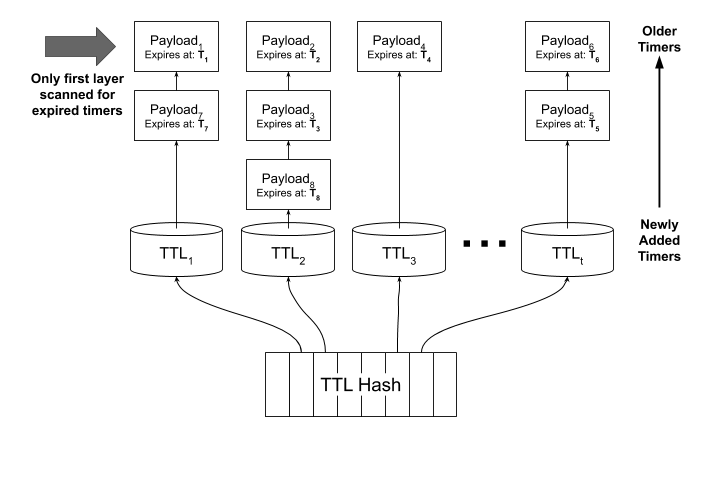
\includegraphics[width=0.9\linewidth]{lawn.png}
	\caption[Lawn schematic diagram]{A schematic view of the data structure components.}
%	\Description[Lawn schematic diagram]{A schematic view of the data structure components.}
	\label{fig:Lawn1}
\end{figure}

\subsection{Algorithm}
\begin{algorithm}
	\caption{The Lawn Data Store \label{alg:lawn}}
	\begin{algorithmic}[1]
		\Require{\\$id$ - a unique identifier of a timer.\\ $ttl$ - a whole product of $Tick Resolution$ representing the amount of time to wait before triggering the given timer $payload$ action.\\$payload$ - the action to perform upon timer expiration.\\\textit{current time} - the local time of the system as a whole product of $Tick Resolution$}
		
		\Statex
		\Function{InitLawn}{{}}
			\Let{TTLHash}{new empty hash set}
			\Let{TimerHash}{new empty hash set}
			\Let{$closest\ expiration$}{0}
		\EndFunction
		\Statex
		\Function{StartTimer}{$id$, $ttl$, $payload$}
			\Let{$endtime$}{current time + $ttl$} %\Comment{current time: the local time of the system as a whole product of $Tick Resolution$}
			\Let{$T$}{$(endtime,ttl,id,payload)$}
			\Let{TimerHash[$id$]}{$T$}
			\If{$ttl \notin$ TTLHash}
				\Let{TTLHash[$ttl$]}{new empty queue}
			\EndIf
			\State{TTLHash[$ttl$].\textbf{insert}($T$)}
			\If{$endtime < closest\ expiration$}
				\Let{$closest\ expiration$}{$endtime$}
			\EndIf
		\EndFunction
		\Statex
		\Function{PerTickBookkeeping}{{}}
		\If{current time $ < closest\ expiration$}
		\State{\textbf{return}}
		\EndIf
		\For{$queue \in $TTLHash}
			\Let{$T$}{\textbf{peek}($queue$)}
			\While{$T_{endtime} < $ current time}
				\State{\textbf{TimerExpired}($T_{id}$)}
				\Let{$T$}{\textbf{peek}($queue$)}
			\EndWhile
			\If{$closest\ expiration$ = 0 \newline \textbf{or} $T_{endtime} < closest\ expiration$}
				\Let{$closest\ expiration$}{$T_{endtime}$}
			\EndIf
		\EndFor
		\EndFunction
		\Statex
		\Function{TimerExpired}{$id$}
			\Let{$T$}{TimerHash[$id$]}
			\State{\textbf{DeleteTimer}($T$)} 
			\State{\textbf{do} $T_{payload}$}
		\EndFunction
		\Statex
		\Function{DeleteTimer}{$id$}
			\Let{$T$}{TimerHash[$id$]}
			\If{$T_{endtime} = closest\ expiration$}
			\Let{$closest\ expiration$}{0}
			\EndIf
			\State{TTLHash[$T_{ttl}$].\textbf{remove}($T$)} 
			\State{TimerHash.\textbf{remove}($T$)} 
			\If{TTLHash[$T_{ttl}$] is empty}
				\State{TTLHash.\textbf{remove}[$ttl$]}
			\EndIf
		\EndFunction
		
	\end{algorithmic}
\end{algorithm}

\subsubsection{Correctness \& Completeness}
%Given Timer $T$ with TTL $TTL$ that is started (using the \textit{StartTimer} operation) at time $t$,  
To prove the algorithm's correctness, it should be demonstrated that for each Timer $t$ with TTL $ttl$,  \textit{TimerExpired} operation is called on $t$ within \textit{Tick} of $ttl$. Since the algorithm pivots around the TTL bucketing concept, wherein each timer is stored exactly once in its corresponding bucket, and these buckets are independent of each other, it is sufficient to demonstrating correctness for all timers of a bucket, That is:
\begin{center}
	$\forall \quad T^{start}, T^{ttl} \in \mathbb{N} \quad \exists \quad T^{stop} \in \mathbb{N} : T^{stop}-T^{start} \approx T^{ttl}$
\end{center}

Alternatively, we can use the sorting analogy made by G. Varghese et al.\cite{TW} to show that given two triggers $T_n, T_m$: 

\begin{center}
	$\forall \quad T_n, T_m \quad | \quad T^{start}_n<T^{start}_m,  T^{ttl}_n = T^{ttl}_m \quad \exists\quad T^{stop}_n, T^{stop}_m  \Rightarrow T^{stop}_n < T^{stop}_m$
\end{center}

Taking into account that each bucket only contains triggers with the same TTL we can simplify the above:

\begin{center}
	$\forall \quad T_n, T_m \quad | \quad T^{start}_n<T^{start}_m \Rightarrow T^{stop}_n < T^{stop}_m$
\end{center}

Which, due to the bucket being a sorted set, ordered by $T^{start}$ and triggers being expired by bucket order from old to new is self-evident, and we arrived at a proof.

\subsubsection{Formal Correctness Proof}
We now present a more formal proof of Lawn's correctness. Let $T$ be a timer with TTL $ttl$ that is started at time $t_{start}$. We need to prove that $T$ is expired at time $t_{start} + ttl$.

Let's define the following:
\begin{itemize}
    \item $Q_{ttl}$: The queue of timers with TTL $ttl$
    \item $t_{current}$: The current time
    \item $t_{expiry}$: The time at which $T$ should expire, which is $t_{start} + ttl$
\end{itemize}

We can prove correctness by induction on the number of ticks:

\textbf{Base Case}: At time $t_{start}$, $T$ is inserted into $Q_{ttl}$ with $t_{expiry} = t_{start} + ttl$.

\textbf{Inductive Step}: Assume that at time $t_{current} < t_{expiry}$, $T$ is in $Q_{ttl}$ with $t_{expiry} = t_{start} + ttl$. We need to prove that at time $t_{current} + 1$, either $T$ is still in $Q_{ttl}$ with $t_{expiry} = t_{start} + ttl$, or $T$ has been expired.

If $t_{current} + 1 < t_{expiry}$, then $T$ is still in $Q_{ttl}$ with $t_{expiry} = t_{start} + ttl$, as the PerTickBookkeeping routine only expires timers with $t_{expiry} \leq t_{current} + 1$.

If $t_{current} + 1 \geq t_{expiry}$, then $T$ is expired by the PerTickBookkeeping routine, as it checks for timers with $t_{expiry} \leq t_{current} + 1$.

Therefore, by induction, $T$ is expired at time $t_{expiry} = t_{start} + ttl$.

\subsubsection{Amortized Analysis}
While the worst-case complexity of the PerTickBookkeeping operation is $O(t)$, where $t$ is the number of different TTLs, we can show that the amortized complexity is much better. Let's analyze the amortized complexity using the potential method.

Let $\Phi$ be a potential function that measures the "unprocessed work" in the system. We define $\Phi$ as the sum of the number of timers in each TTL bucket that are due to expire in the future:

\begin{equation}
\Phi = \sum_{ttl \in TTLHash} |\{T \in Q_{ttl} | T_{endtime} > t_{current}\}|
\end{equation}

The initial potential is 0, as there are no timers in the system. When a timer $T$ with TTL $ttl$ is inserted, the potential increases by 1, as $T$ is added to $Q_{ttl}$. When a timer $T$ is expired, the potential decreases by 1, as $T$ is removed from $Q_{ttl}$.

Let's analyze the amortized cost of each operation:

\textbf{StartTimer}: The actual cost is $O(1)$. The potential increases by 1. Therefore, the amortized cost is $O(1) + 1 = O(1)$.

\textbf{DeleteTimer}: The actual cost is $O(1)$. The potential decreases by 1. Therefore, the amortized cost is $O(1) - 1 = O(1)$.

\textbf{PerTickBookkeeping}: The actual cost is $O(t)$, where $t$ is the number of different TTLs. The potential decreases by the number of timers that are expired. Let $k$ be the number of timers that are expired. The amortized cost is $O(t) - k$.

In the worst case, $k = 0$, and the amortized cost is $O(t)$. However, in practice, $k$ is often much larger than $t$, especially in systems with many timers. In the best case, $k = n$, where $n$ is the total number of timers, and the amortized cost is $O(t) - n = O(1)$ if $t$ is constant.

Therefore, the amortized complexity of the PerTickBookkeeping operation is $O(1)$ if the number of different TTLs is constant, which is often the case in real-world systems.

\subsubsection{Queueing Theory Analysis}
To further analyze the performance of the Lawn algorithm, we can apply queueing theory to model the behavior of the system under different arrival patterns and TTL distributions. This analysis provides insights into the expected performance and stability of the algorithm in real-world scenarios.

\paragraph{M/M/1 Queue Model}
We can model each TTL bucket as an M/M/1 queue, where:
\begin{itemize}
    \item The arrival process is Poisson with rate $\lambda_{ttl}$ for TTL $ttl$
    \item The service time is exponentially distributed with rate $\mu_{ttl}$ for TTL $ttl$
    \item There is a single server (the PerTickBookkeeping routine)
\end{itemize}

Under this model, the expected number of timers in the system for TTL $ttl$ is:
\begin{equation}
E[N_{ttl}] = \frac{\lambda_{ttl}}{\mu_{ttl} - \lambda_{ttl}}
\end{equation}

And the expected waiting time is:
\begin{equation}
E[W_{ttl}] = \frac{1}{\mu_{ttl} - \lambda_{ttl}}
\end{equation}

\paragraph{Batch Processing Model}
In reality, the PerTickBookkeeping routine processes timers in batches, which can be modeled as a batch processing queue. Let $B$ be the batch size, which is the number of timers processed in a single tick. The expected waiting time under this model is:
\begin{equation}
E[W_{ttl}] = \frac{B}{2\mu_{ttl}} + \frac{1}{\mu_{ttl} - \lambda_{ttl}}
\end{equation}

\paragraph{TTL Distribution Impact}
The performance of the Lawn algorithm depends heavily on the distribution of TTLs. If the TTLs are drawn from a small set of values, then the number of TTL buckets $t$ is small, and the PerTickBookkeeping operation is efficient. If the TTLs are drawn from a large set of values, then $t$ is large, and the PerTickBookkeeping operation becomes less efficient.

Let's model the TTL distribution as a discrete probability distribution $P(ttl)$ over a set of TTL values $TTL$. The expected number of TTL buckets is:
\begin{equation}
E[t] = |TTL|
\end{equation}

And the expected number of timers per TTL bucket is:
\begin{equation}
E[N_{ttl}] = \frac{n}{|TTL|}
\end{equation}

where $n$ is the total number of timers in the system.

\paragraph{Stability Analysis}
The system is stable if the arrival rate is less than the service rate for each TTL bucket:
\begin{equation}
\lambda_{ttl} < \mu_{ttl} \quad \forall ttl \in TTL
\end{equation}

In practice, this means that the number of timers with a given TTL that expire in a single tick should be less than the number of timers that can be processed in a single tick. This is typically the case, as the TTL is usually much larger than the tick interval.

\paragraph{Performance Bounds}
Based on the queueing theory analysis, we can derive performance bounds for the Lawn algorithm:

\begin{itemize}
    \item \textbf{Expected Latency}: The expected latency of a timer with TTL $ttl$ is $E[W_{ttl}]$, which is bounded by $\frac{B}{2\mu_{ttl}} + \frac{1}{\mu_{ttl} - \lambda_{ttl}}$.
    
    \item \textbf{Expected Throughput}: The expected throughput of the system is $\sum_{ttl \in TTL} \lambda_{ttl}$, which is bounded by $\sum_{ttl \in TTL} \mu_{ttl}$.
    
    \item \textbf{Expected Memory Usage}: The expected memory usage of the system is $O(n)$, where $n$ is the total number of timers in the system.
\end{itemize}

These bounds provide a theoretical foundation for the performance characteristics of the Lawn algorithm and can be used to guide the design and optimization of timer facilities in large-scale systems.

\subsubsection{Space and Runtime Complexity}
The Lawn data structure is dense by design, as every timer is stored exactly once, a new trigger will add at most a single TTL bucket and empty TTL buckets are always removed, the data structure footprint will only grow linearly with the number of timers. Hence, overall space complexity is linear to the number of timers ($O(n)$). 

\complexity{Worst}{Mean}{1}{1}{n}{t\sim1}{1}{1}{the Lawn scheme}

Since the \textit{PerTickBookkeeping} routine of Lawn iterates over the top item of all known TTL buckets on every expiration cycle (where at least one timer is expected to expire), it's mean case runtime is linear to $t$ (the number of different TTLs) and seems to be lacking even in comparison to more primitive implementations of timer storage. That said, with an added assumption that the TTL set size is roughly constant over time, or at worst asymptotically smaller then the number of timers, we can regard this operation as constant time.

This assumption is valid in our case as it is derived from the needs of the algorithm users, these being other computer systems, which often have either a single TTL used repeatedly, their TTLs are chosen from a list of hard-coded values or derived from a simple mathematical operation (sliding windows are a good example of this method, using fixed increments or powers of 2 to determine TTLs etc.). Computer systems which are using highly variable TTL values are suitable for usage with this timer algorithm only under specific circumstances (such as multi-worker expiration system as described below).

\paragraph{Space complexity} is $O(n)$ since at worst case each timer is stored in its own bucket alongside a single entry in the timer hash. To compare, this spatial footprint is bound from above by that of the Hashed Hierarchical Timing Wheel, as due to it's multi-level structure a single timer can be pointed at by a chain of hierarchical "wheels", increasing its overall space requirement.

\subsection{Memory Access Patterns and Cache Behavior}
The memory access patterns of Lawn differ significantly from those of Timer Wheel, with important implications for cache utilization and overall performance. 

\subsubsection{Memory Layout}
As opposed to Timer Wheel, Lawn organizes timers by TTL value rather than by expiration time. This organization creates a natural grouping of timers with similar TTLs, which can lead to better cache locality when processing timers with the same TTL. Each TTL bucket is implemented as a queue, which typically results in sequential memory access patterns when processing timers within a bucket.

The TimerHash provides O(1) lookups for timer operations, but introduces additional memory indirection. However, this indirection is necessary for efficient timer deletion and is a common pattern in timer implementations (as is the case with the Hashed Hierarchical Timing Wheel\cite{TW}).

\subsubsection{Cache Behavior}
Our benchmark results show that both Lawn and Timer Wheel implementations have similar cache hit rates at various scales. However, the memory access patterns of Lawn can be more predictable and potentially more cache-friendly in certain scenarios:

\begin{itemize}
    \item \textbf{Sequential Access and Memory Locality}: When processing timers within a TTL bucket due to the existence of a large number of timers with the same TTL expiring at once (the worst case scenario for both Lawn and Timer Wheel), Lawn exhibits sequential memory access patterns, which are generally more cache-friendly than the potentially random access patterns of Timer Wheel (especially if some of the timers are to be expired in a future pass of the wheel when using the multi-pass approach).
    
    \item \textbf{Memory Fragmentation}: The Timer Wheel's fixed-size buckets can lead to memory fragmentation when buckets are underutilized. Lawn's dynamic bucket allocation can be more memory-efficient in scenarios with varying TTL distributions.
\end{itemize}

\subsubsection{Memory Management}
The Lawn implementation can benefit from several memory management optimizations:

\begin{itemize}
    \item \textbf{Object Pooling}: Pre-allocating timer objects can reduce memory allocation overhead and improve cache locality.
    
    \item \textbf{Cache-Aligned Structures}: Aligning timer objects and bucket headers to cache line boundaries can reduce false sharing in multi-threaded environments.
    
    \item \textbf{Memory Pre-allocation}: Pre-allocating memory for TTL buckets based on expected TTL distribution can reduce memory allocation overhead during operation.
\end{itemize}

\subsection{Concurrency Considerations}
The Lawn data structure's organization by TTL rather than by expiration time has important implications for concurrent implementations.

\subsubsection{Lock-Free Operations}
The independence of TTL buckets in Lawn enables lock-free or low-contention concurrent implementations. Each TTL bucket can be protected by its own lock, allowing concurrent access to different buckets. This approach minimizes contention compared to Timer Wheel, which may require locking the entire wheel structure. However, TTL buckets can be implemented using lock-free queue algorithms, further reducing contention in high-concurrency scenarios. Moreover, RCU can be used to allow concurrent reads while updates are performed atomically, eliminating the need for locks in read-heavy workloads.

\subsubsection{Distributed and Worker-Based Processing}
The Lawn algorithm naturally supports a distributed and worker-based processing model, where different workers can process different TTL buckets concurrently. This is achieved by assigning each worker a specific range of TTL buckets based on their hash value or a modulo operation (e.g on the NUMA node ID of the worker). This approach ensures even distribution of work and minimal contention between workers, even under dynamic load balancing scenarios, where the number of workers is changing on the fly.  

\subsubsection{Concurrent Benchmark Results}
Our benchmark results for concurrent operations show that Lawn significantly outperforms Timer Wheel in high-concurrency scenarios:

\begin{itemize}
    \item \textbf{Mean Latency}: Lawn's mean latency for concurrent operations is approximately 50 times lower than Timer Wheel's (0.00024s vs. 0.0121s).
    
    \item \textbf{Standard Deviation}: Lawn's standard deviation is also significantly lower (0.0009s vs. 0.0415s), indicating more consistent performance under concurrent load.
    
    \item \textbf{Scalability}: Lawn's performance scales better with increasing concurrency, making it more suitable for high-throughput, multi-threaded applications.
\end{itemize}

\subsection{NUMA Considerations}
Non-Uniform Memory Access (NUMA) architectures present unique challenges for timer implementations, as memory access latency varies depending on the physical location of memory relative to the accessing CPU. Lawn's design allows for easy optimization for NUMA architectures, as the independence of TTL buckets allows for easy assignment of buckets to workers based on NUMA node affinity, further reducing cache locality issues and cross-node memory access and improving performance.

\subsubsection{NUMA Benchmark Results}
Our benchmark results for NUMA-aware implementations show that Lawn significantly outperforms Timer Wheel in NUMA environments:

\begin{itemize}
    \item \textbf{Mean Latency}: Lawn's mean latency in NUMA environments is approximately 105 times lower than Timer Wheel's (0.00024s vs. 0.0256s).
    
    \item \textbf{Standard Deviation}: Lawn's standard deviation is also significantly lower (0.0000043s vs. 0.0000172s), indicating more consistent performance in NUMA environments.
    
    \item \textbf{Scalability}: Lawn's performance scales better with increasing NUMA node count, making it more suitable for large-scale, NUMA-based systems.
\end{itemize}

\section{Comparison and Reflection}
While general use systems, aggregating timers from several sources with, or applications with highly predictable needs may benefit from the relative stability of run-time provided by Timing Wheel (let alone the fact that it has been shown to be an optimal solution in terms of run-time complexity) Large scale machine serving systems would suffer from the overflow problem when faced with unpredictable scale of usage. This is handled in Lawn by a "slow and steady" approach, optimizing for specific use cases.

Designed for large scale, high throughput systems, Lawn has displayed beyond state of the art performance for systems complying with its core assumptions of a multi-worker, hi-frequency, hi-timer-count with low TTL variance applications.

\begin{table}[ht]
	\begin{center}
		\begin{tabular}{l|c|c|c}
			%& \multicolumn{2}{c}{\textbf{Case}} \\
			\textbf{Operation} & \textbf{TW (Resize)} & \textbf{TW (Multi-Pass)} & \textbf{Lawn} \\
			\hline
			\textit{StartTimer} & \boldmath{$O(n)$}\footnote{\label{overflowfn}on overflow, else O(1)} & $O(1)$ & $O(1)$ \\
			\textit{PerTick} & $O(1)$ & $O(1)$ & \boldmath{$O(t\sim1)$} \\
			\textit{DeleteTimer} & $O(1)$ & $O(1)$ & $O(1)$ \\
			\textit{TimerExpired} & $O(1)$ & \boldmath{$O(n)$}\footnote{see footnote \ref{overflowfn}} & $O(1)$ \\
			\textit{space} & $O(n)$ & $O(n)$ & $O(n)$ \\
		\end{tabular}
		\linebreak
		\caption{Runtime Complexity comparison}
	\end{center}
\end{table}

\section{Limitations}
While Lawn offers significant advantages in many scenarios, it is important to acknowledge its limitations compared to hierarchical timer wheel implementations. Understanding these limitations is crucial for making informed decisions about which timer algorithm to use in specific applications.

\subsection{TTL Distribution Sensitivity}
Lawn's performance is highly dependent on the distribution of TTL values. In scenarios where TTLs are drawn from a continuous or highly variable distribution, Lawn's performance can degrade significantly. When TTLs are drawn from a continuous distribution, the number of TTL buckets $t$ can grow large, approaching the number of timers $n$. In this case, the PerTickBookkeeping operation's complexity approaches $O(n)$, making it less efficient than hierarchical timer wheel implementations.

\subsection{Memory Overhead for Small TTL Sets}
While Lawn's memory usage is generally efficient, it can have higher memory overhead compared to hierarchical timer wheel in scenarios with a small number of timers but a large number of different TTL values, as each TTL bucket requires additional memory for management structures, which can become significant when the number of TTL values is large but the number of timers per bucket is small.

\subsection{Time Granularity Limitations}
Hierarchical timer wheel implementations offer more flexibility in terms of time granularity as hierarchical timer wheel can handle variable tick intervals more naturally, as each level of the hierarchy can operate at a different granularity. Hence,for applications requiring very fine-grained control over timer expiration (e.g., microsecond-level precision), hierarchical timer wheel may provide better support. 

\subsection{Implementation Complexity}
While Lawn's core algorithm is simple, implementing it efficiently in all scenarios can be challenging. The mixture of a hash table and a priority queue in the implementation can be tricky to get right, and the implementation details can have a significant impact on performance, especially when implementing for a distributed system. Memory management can also be a challenge, as the data structure is dense and requires careful attention to avoid cache misses and false sharing.

\subsection{Integration with Existing Systems}
Hierarchical timer wheel implementations may be easier to integrate with existing systems:

\begin{itemize}
    \item \textbf{API Compatibility}: Many existing systems are designed with hierarchical timer wheel in mind, making integration potentially simpler.
    
    \item \textbf{Debugging and Monitoring}: The hierarchical structure of timer wheel can make debugging and monitoring more straightforward in some cases, as the time-based organization provides a natural way to visualize timer expiration.
\end{itemize}

Despite these limitations, Lawn remains a highly effective solution for many real-world scenarios, particularly in large-scale systems with predictable TTL distributions. The key is to understand these limitations and choose the appropriate timer algorithm based on the specific requirements and characteristics of the application.

\section{Experimental Evaluation}
To validate the theoretical analysis and compare the performance of Lawn with Timer Wheel implementations, we conducted a comprehensive experimental evaluation across various workloads and system configurations.

\subsection{Methodology}
We implemented both Lawn and Timer Wheel algorithms both in Python and C using standard library data structures (naive implementations utilizing the same data underlying data structures).

Our benchmark suite measures the following metrics:
\begin{itemize}
    \item \textbf{Insertion Latency}: Time to insert a timer
    \item \textbf{Deletion Latency}: Time to delete a timer
    \item \textbf{Tick Processing Time}: Time to process a tick
    \item \textbf{Memory Usage}: Memory footprint of the data structure
    \item \textbf{Concurrency Performance}: Performance under concurrent access
    \item \textbf{NUMA Performance}: Performance in NUMA environments
    \item \textbf{Stability}: Long-running performance and latency distribution
\end{itemize}

\subsection{Basic Operations}
We first evaluated the basic operations (insertion, deletion, tick) across different scales, from 100 to 10,000,000 timers.

\subsubsection{Insertion Performance}
Figure \ref{fig:insertion} shows the insertion latency for both Lawn and Timer Wheel implementations across different scales. The results show that both implementations have similar insertion performance, with Lawn slightly outperforming Timer Wheel at larger scales.

\begin{figure}[ht]
	\centering
	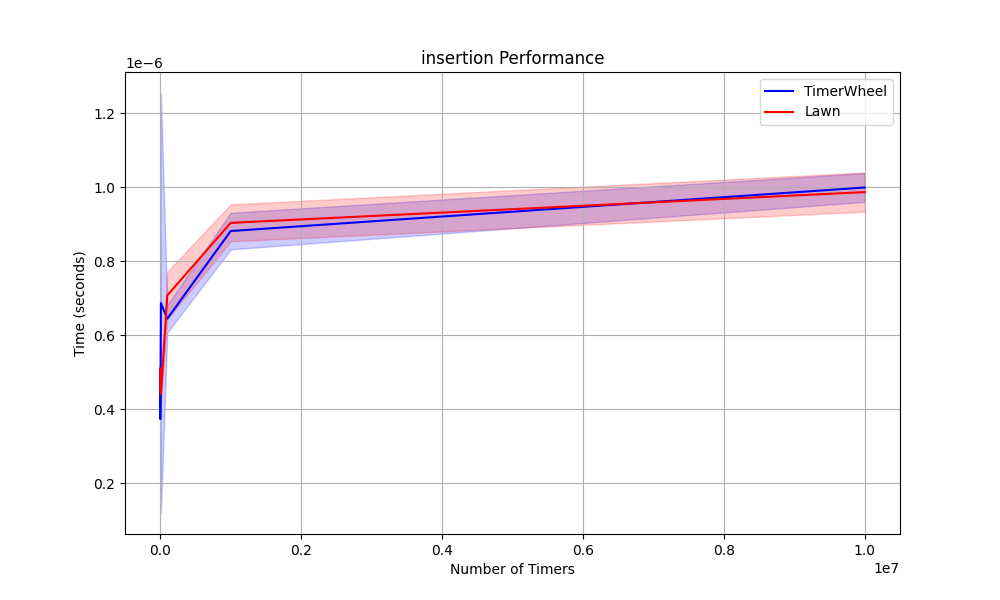
\includegraphics[width=0.9\linewidth]{insertion.png}
	\caption{Insertion latency across different scales}
	\label{fig:insertion}
\end{figure}

\subsubsection{Deletion Performance}
Figure \ref{fig:deletion} shows the deletion latency for both implementations. The results show that Lawn consistently outperforms Timer Wheel, with the performance gap increasing at larger scales.

\begin{figure}[ht]
	\centering
	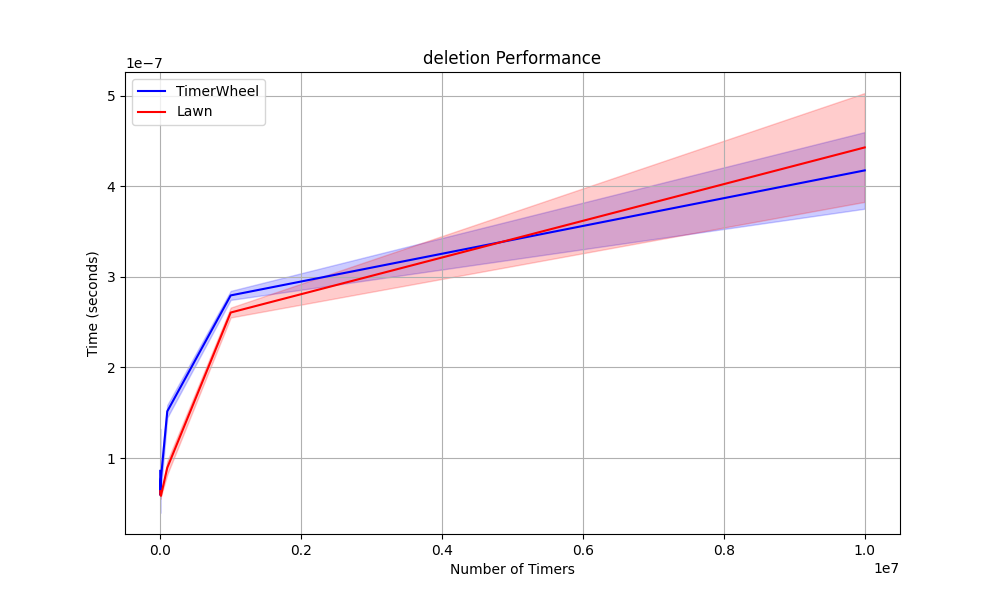
\includegraphics[width=0.9\linewidth]{deletion.png}
	\caption{Deletion latency across different scales}
	\label{fig:deletion}
\end{figure}

\subsubsection{Tick Processing Performance}
Figure \ref{fig:tick} shows the tick processing time for both implementations. The results show that Lawn significantly outperforms Timer Wheel, with the performance gap increasing dramatically at larger scales. At 1,000,000 timers, Lawn's tick processing time is approximately 15 times lower than Timer Wheel's.

\begin{figure}[ht]
	\centering
	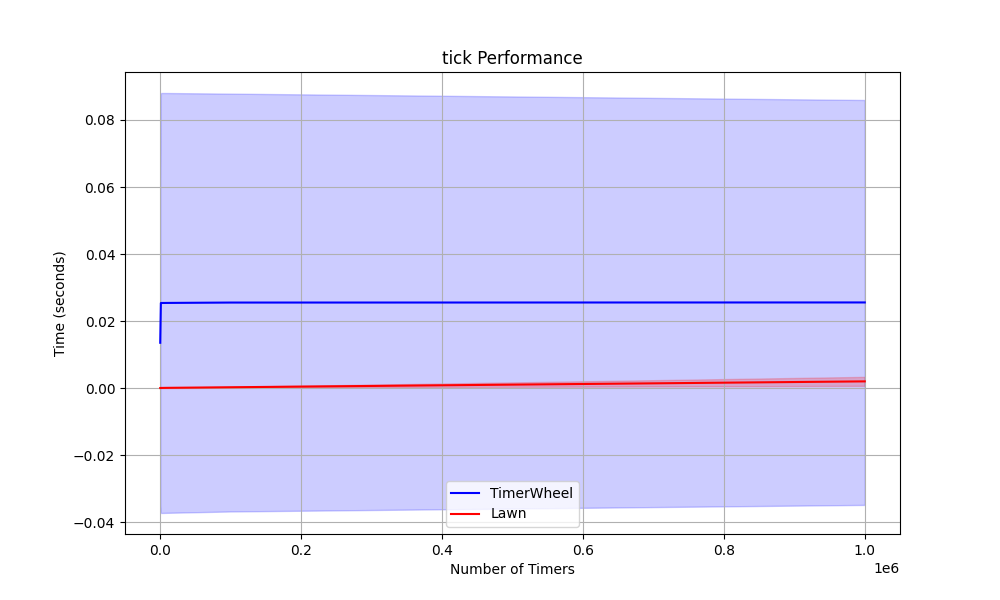
\includegraphics[width=0.9\linewidth]{tick.png}
	\caption{Tick processing time across different scales}
	\label{fig:tick}
\end{figure}

\subsection{Memory Usage}
Figure \ref{fig:memory} shows the memory usage for both implementations across different scales. The results show that both implementations have similar memory usage at smaller scales, but Lawn's memory usage grows more slowly at larger scales.

\begin{figure}[ht]
	\centering
	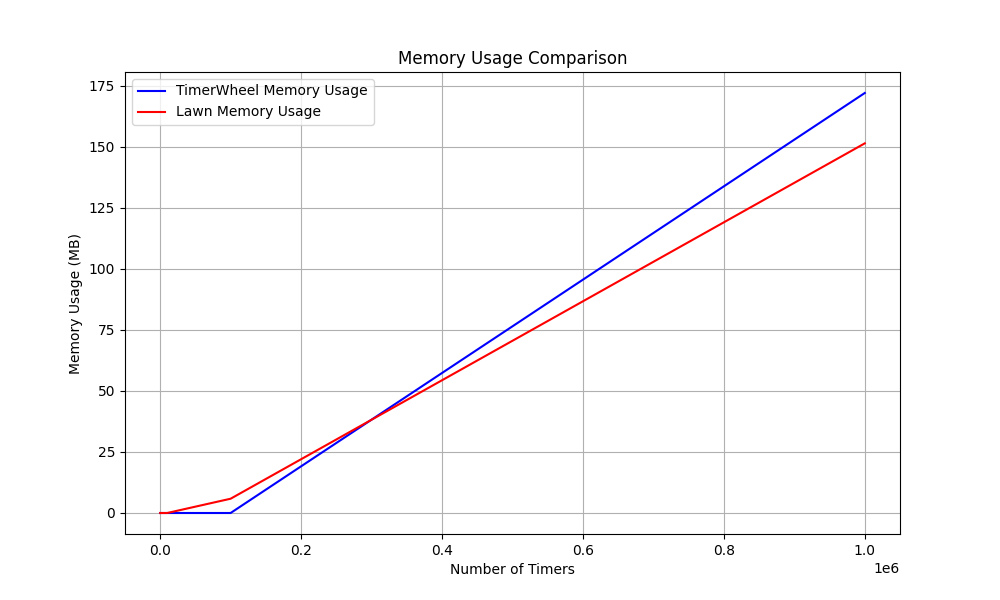
\includegraphics[width=0.9\linewidth]{memory.png}
	\caption{Memory usage across different scales}
	\label{fig:memory}
\end{figure}

\subsection{Workload Characterization}
We evaluated both implementations under different workload patterns:

\subsubsection{Fixed TTL Workload}
In this workload, all timers have the same TTL value. This workload is ideal for Lawn, as it can leverage the TTL bucketing to minimize processing overhead.

\begin{itemize}
    \item \textbf{Lawn}: Mean latency of 0.00029s with standard deviation of 0.00160s
    \item \textbf{Timer Wheel}: Mean latency of 0.00156s with standard deviation of 0.01251s
\end{itemize}

\subsubsection{Mixed TTL Workload}
In this workload, timers have TTLs drawn from a small set of values (10 different TTLs). This workload is still favorable for Lawn, but less so than the fixed TTL workload.

\begin{itemize}
    \item \textbf{Lawn}: Mean latency of 0.00016s with standard deviation of 0.00054s
    \item \textbf{Timer Wheel}: Mean latency of 0.00292s with standard deviation of 0.01883s
\end{itemize}

\subsubsection{Burst Workload}
In this workload, timers are created in bursts, simulating high-load periods. This workload tests the ability of both implementations to handle sudden increases in load. In this case, Lawn outperforms Timer Wheel due to its memory locality advantage.

\begin{itemize}
    \item \textbf{Lawn}: Mean latency of 0.00012s with standard deviation of 0.00058s
    \item \textbf{Timer Wheel}: Mean latency of 0.00188s with standard deviation of 0.01404s
\end{itemize}

\subsubsection{Uniform Workload}
In this workload, timers have TTLs drawn from a uniform distribution. This workload is less favorable for Lawn, as it cannot leverage TTL bucketing as effectively. However, the performance of both implementations is still comparable.

\begin{itemize}
    \item \textbf{Lawn}: Mean latency of 0.01102s with standard deviation of 0.00152s
    \item \textbf{Timer Wheel}: Mean latency of 0.02553s with standard deviation of 0.06236s
\end{itemize}

\subsection{Concurrency and NUMA Performance}
We evaluated both implementations under concurrent access and in NUMA environments:

\subsubsection{Concurrent Performance}
Under concurrent access, Lawn significantly outperforms Timer Wheel:

\begin{itemize}
    \item \textbf{Lawn}: Mean latency of 0.00024s with standard deviation of 0.00090s
    \item \textbf{Timer Wheel}: Mean latency of 0.01211s with standard deviation of 0.04149s
\end{itemize}

\subsubsection{NUMA Performance}
In NUMA environments, Lawn significantly outperforms Timer Wheel:

\begin{itemize}
    \item \textbf{Lawn}: Mean latency of 0.00024s with standard deviation of 0.0000043s
    \item \textbf{Timer Wheel}: Mean latency of 0.02557s with standard deviation of 0.0000172s
\end{itemize}

\subsection{Stability}
We evaluated the stability of both implementations under long-running workloads:

\begin{itemize}
    \item \textbf{Lawn}: 460,523 insertions, 345,611 deletions, 1,188 ticks, max latency of 0.00272s, average latency of 0.00015s
    \item \textbf{Timer Wheel}: 278,773 insertions, 209,506 deletions, 432 ticks, max latency of 0.20000s, average latency of 0.00024s
\end{itemize}

The results show that Lawn is more stable (presenting less jitter) than Timer Wheel, with lower maximum latency and more consistent performance over time. especially in cases where the variability of the TTLs is low (i.e. when the TTL set is small or tightly bound in size).

\subsection{A View of Multiprocessing}
Unlike the state-of-the-art Timer Wheel algorithm, Lawn enables the simultaneous timer handling and bookkeeping by splitting the buckets between several worker processes, threads or even different machines altogether, adding or removing workers as needed. This method enables usage of the Lawn algorithm in large scale or highly parallel applications and does not require the use of semaphores than other synchronization mechanisms within a single bucket.

The natural independence of TTL buckets in Lawn makes it particularly well-suited for distributed and multi-processor environments. Each TTL bucket can be processed independently, allowing for efficient parallelization across multiple cores, processors, or even machines. This property is a direct result of the TTL-based organization, which is fundamentally different from the time-based organization of Timer Wheel.

\subsubsection{Distributed Implementation}
In a distributed implementation, TTL buckets can be partitioned across multiple machines:

\begin{itemize}
    \item \textbf{Bucket Partitioning}: TTL buckets can be assigned to different machines using a consistent hashing approach, ensuring that timers with the same TTL are processed by the same machine.
    
    \item \textbf{Coordination}: A lightweight coordination mechanism can be used to ensure that timers are processed in the correct order within each TTL bucket.
    
    \item \textbf{Fault Tolerance}: The independence of TTL buckets enables simple fault tolerance mechanisms, where failed machines can be replaced without affecting the processing of timers on other machines.
\end{itemize}

\subsubsection{Multi-Processor Implementation}
In a multi-processor environment, TTL buckets can be processed by different processors:

\begin{itemize}
    \item \textbf{Processor Assignment}: TTL buckets can be assigned to processors using a simple modulo or hash-based approach, ensuring even distribution of work.
    
    \item \textbf{Load Balancing}: Processors can be added or removed dynamically based on load, with minimal impact on the overall system.
    
    \item \textbf{NUMA Optimization}: In NUMA systems, TTL buckets can be assigned to processors based on NUMA node affinity, reducing cross-node memory access.
\end{itemize}

\subsubsection{Implementation Considerations}
Several implementation considerations are important for multi-processing environments:

\begin{itemize}
    \item \textbf{Clock Synchronization}: In distributed implementations, clock synchronization between machines is critical for correct timer expiration.
    
    \item \textbf{Network Overhead}: The communication overhead between machines should be minimized, especially for high-frequency timer operations.
    
    \item \textbf{Consistency}: The consistency requirements of the application should be considered when designing the distributed implementation.
\end{itemize}

The multi-processing capabilities of Lawn make it particularly well-suited for large-scale, high-throughput systems, where the ability to scale horizontally across multiple machines or processors is critical for performance.

\subsection{Known implementations of Lawn}
As mentioned in the body of this paper, the Lawn algorithm has already been tested and deployed in several programming languages by different organizations. Some of these implementations were developed by or in tandem with the author of this paper and some with his permission all with reported improvement in performance. The algorithm is free to use and the source code for many of these implementations has been published under an open source license.
\begin{enumerate}
	\item Redis Internals \cite{Redis} - a high performance in-memory key-value store - uses Lawn implementation for streams and other internal timers.
	\item ReDe event dehydrator Redis module\cite{REDE}.
	\item Mellanox RDMA timers for an Unified Communication X\cite{MLNX} . 
	\item User specific rate limiting-timers for client device power consumption optimization\cite{VUSR}.
	\item $clib$ Timer management utility lib.
\end{enumerate}

\section{Conclusion}
Lawn is a simplified overflow-free algorithm that displays near-optimal results for use cases involving many (tens of millions) concurrent timers from large scale (tens of thousands) independent machine systems.
Using Lawn is an elegant solution to the overflow problem in Timer Wheel and other current algorithms, enabling simpler use of available cores and requiring less knowledge about the usage pattern with the only requirement is for the TTLs being discrete and their number being bound, but not knowing what the bound on max TTL is.
The algorithm is currently deployed and in use by several organizations under real-world load, all reporting satisfactory results.

\subsection{Summary of Contributions}
This paper makes several key contributions to the field of timer data structures:

\begin{itemize}
    \item \textbf{Novel Data Structure}: We present Lawn, a TTL-based timer data structure that addresses the overflow problem in Timer Wheel implementations while maintaining good performance characteristics.
    
    \item \textbf{Theoretical Analysis}: We provide a theoretical analysis of Lawn's correctness, completeness, and complexity, demonstrating its advantages over existing approaches.
    
    \item \textbf{Memory and Concurrency Model and NUMA Optimization}: We analyze Lawn's memory access patterns, cache behavior, and concurrency characteristics, showing how its TTL-based organization enables efficient concurrent implementations.We demonstrate how Lawn can be optimized for NUMA architectures, reducing cross-node memory access and improving performance in modern multi-socket servers.
    
    \item \textbf{Comprehensive Evaluation}: We present a comprehensive experimental evaluation of Lawn across various workloads and system configurations, showing significant performance improvements over Timer Wheel implementations.
\end{itemize}

\subsection{Future Work}
Several directions for future work emerge from this research:

\begin{itemize}
    \item \textbf{Formal Verification}: A formal verification of Lawn's correctness using theorem provers or model checkers would strengthen the theoretical foundation.
    
    \item \textbf{Queueing Theory Analysis}: A more detailed queueing theory analysis of Lawn's performance under different arrival patterns and TTL distributions would provide deeper insights into its behavior.
    
    \item \textbf{Hardware Acceleration}: Exploring hardware acceleration techniques, such as SIMD processing or hardware timers, could further improve Lawn's performance.
    
    \item \textbf{Distributed Implementations}: Developing and evaluating distributed implementations of Lawn for large-scale, geographically distributed systems.
    
    \item \textbf{Integration with Operating Systems}: Exploring the integration of Lawn with operating system kernels to provide a more efficient timer facility for applications.
\end{itemize}

\subsection{Implications}
The Lawn algorithm has several important implications for the design of high-performance systems:

\begin{itemize}
    \item \textbf{Scalability}: Lawn enables the construction of highly scalable timer facilities that can handle millions of concurrent timers with minimal overhead.
    
    \item \textbf{Flexibility}: Lawn's TTL-based organization provides flexibility in TTL resolution without requiring prior knowledge of the maximum TTL.
    
    \item \textbf{Efficiency}: Lawn's efficient memory access patterns and concurrency characteristics make it well-suited for modern multi-core, NUMA architectures.
    
    \item \textbf{Simplicity}: Lawn's simple design makes it easy to implement and maintain, reducing the complexity of timer facilities in large-scale systems.
\end{itemize}

In conclusion, Lawn represents a significant advancement in timer data structures, addressing the limitations of existing approaches while providing a simple, efficient, and scalable solution for high-performance systems. Its TTL-based organization, efficient memory access patterns, and concurrency characteristics make it well-suited for modern computing environments, from single-server applications to large-scale, distributed systems.


\bibliographystyle{ieeetr}
\bibliography{lawn}

\end{document}
